\subsection{Requirements}

\begin{figure}[t]
  \begin{center}
  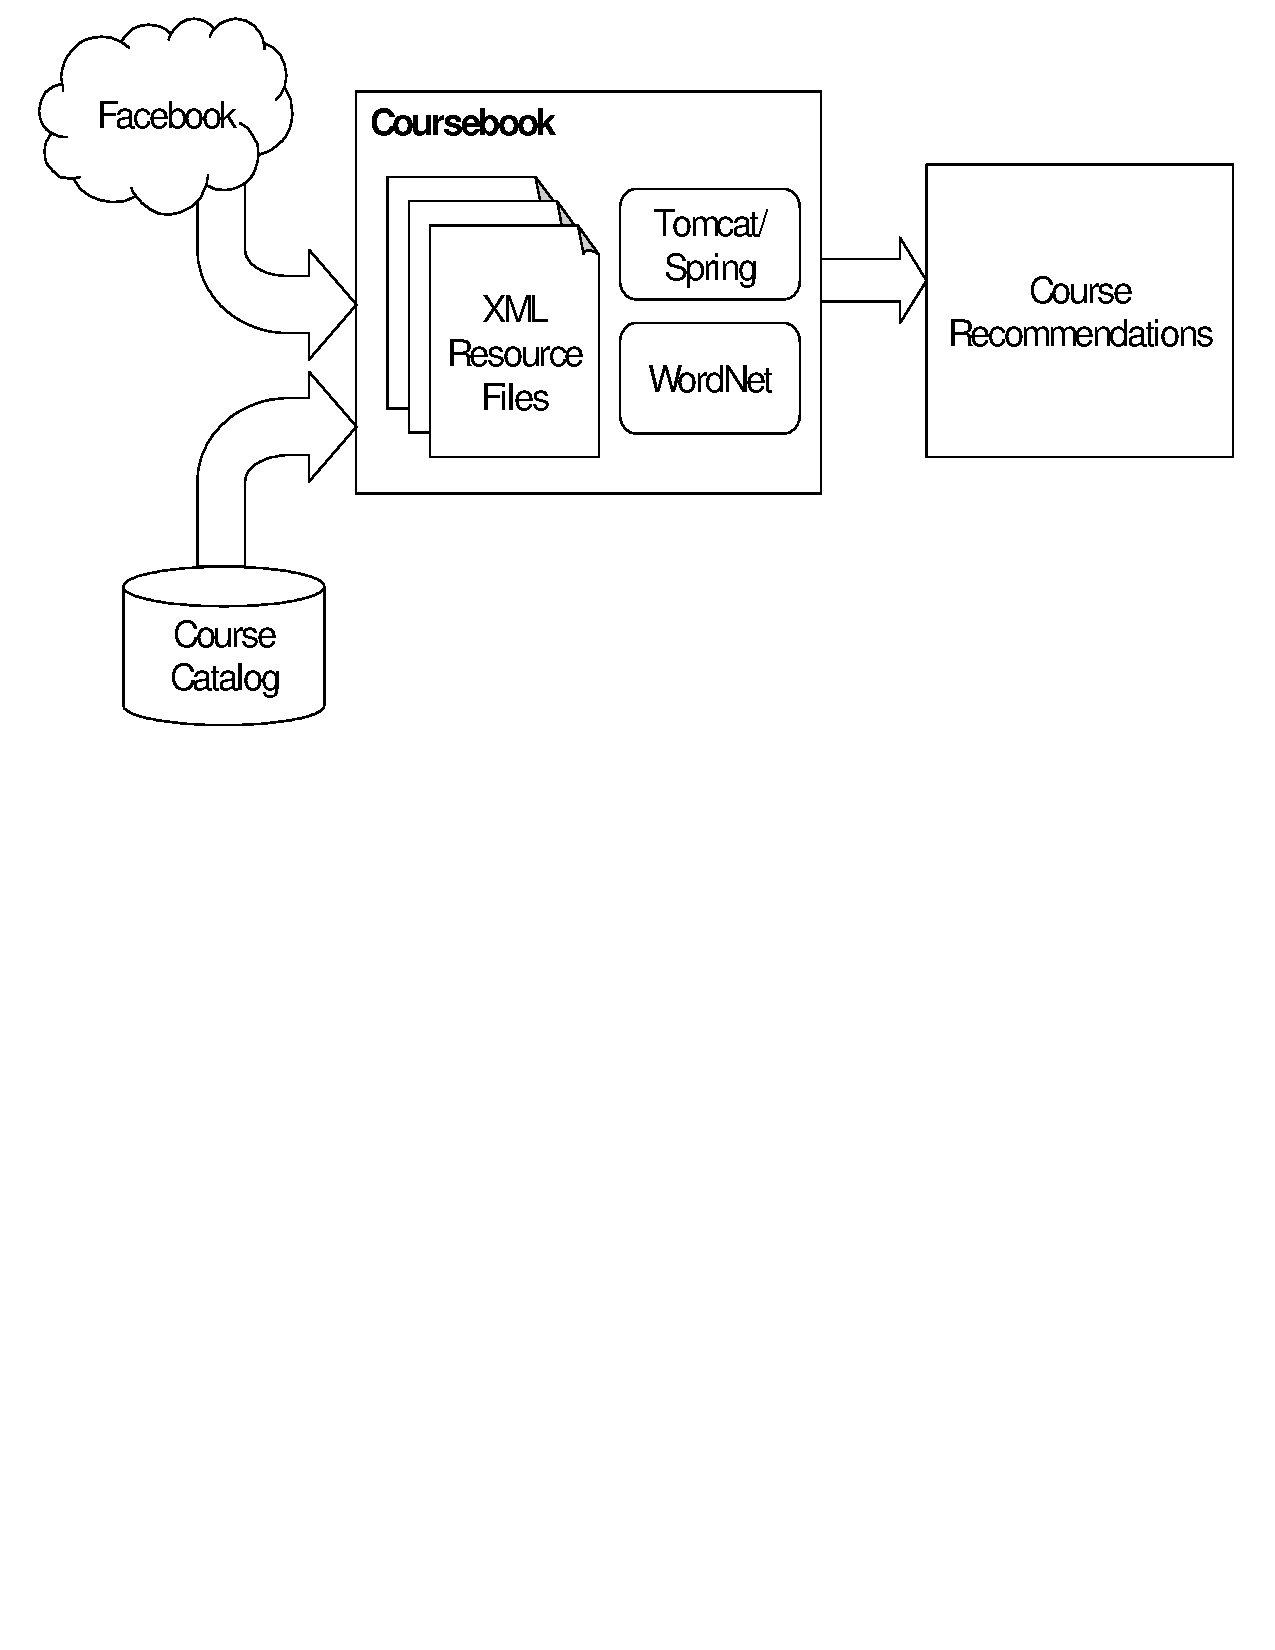
\includegraphics[width=\textwidth]{images/overview}
  \caption{Coursebook Data Flow Overview}
  \label{fig:overview}
  \end{center}
\end{figure}

There are three key requirements necessary for the implementation of Coursebook:
(1) presence of an accessible web-based User Interface, (2) aggregation of live
data from dynamic data sources, and (3) an intelligent querying algorithm to
find relevant course recommendations. Figure \ref{fig:overview} shows how we
achieve these requirements in our implementation. 

\paragraph*{Web User Interface}
By implementing Coursebook with a web-based user interface, we present users 
with an easily accessible service. Coursebook utilizes the latest technologies 
on the J2EE stack, including the Spring framework, JDBC, and WordNet APIs to 
produce a highly responsive system that is platform agnostic on both the server
side (Java) and client side (DHTML/Javascript). This UI is encapsulated in web
forms and the return from the Tomcat servlet container as a list of course
recommendations.

\paragraph*{Live Data}
Coursebook consists of multiple distributed components to provide users with 
information. The system relies on a MySQL database for real-time course catalog
information. The Facebook API provides developers access to its users' profile 
information. Coursebook offers multiple points of entry, including automatic 
Facebook connectivity and manual user input, in case the former system is 
inaccessible.

\paragraph*{Relevant Courses}
Coursebook uses advanced artificial intelligence techniques to search and 
compute the most applicable courses for each individual user. Coursebook's
techniques are obtained by utilizing the WordNet API to both populate the
database with related index terms and to extract and expand keywords from the
user's input.

\subsection{Distributed Components}

\begin{figure}[t]
  \begin{center}
  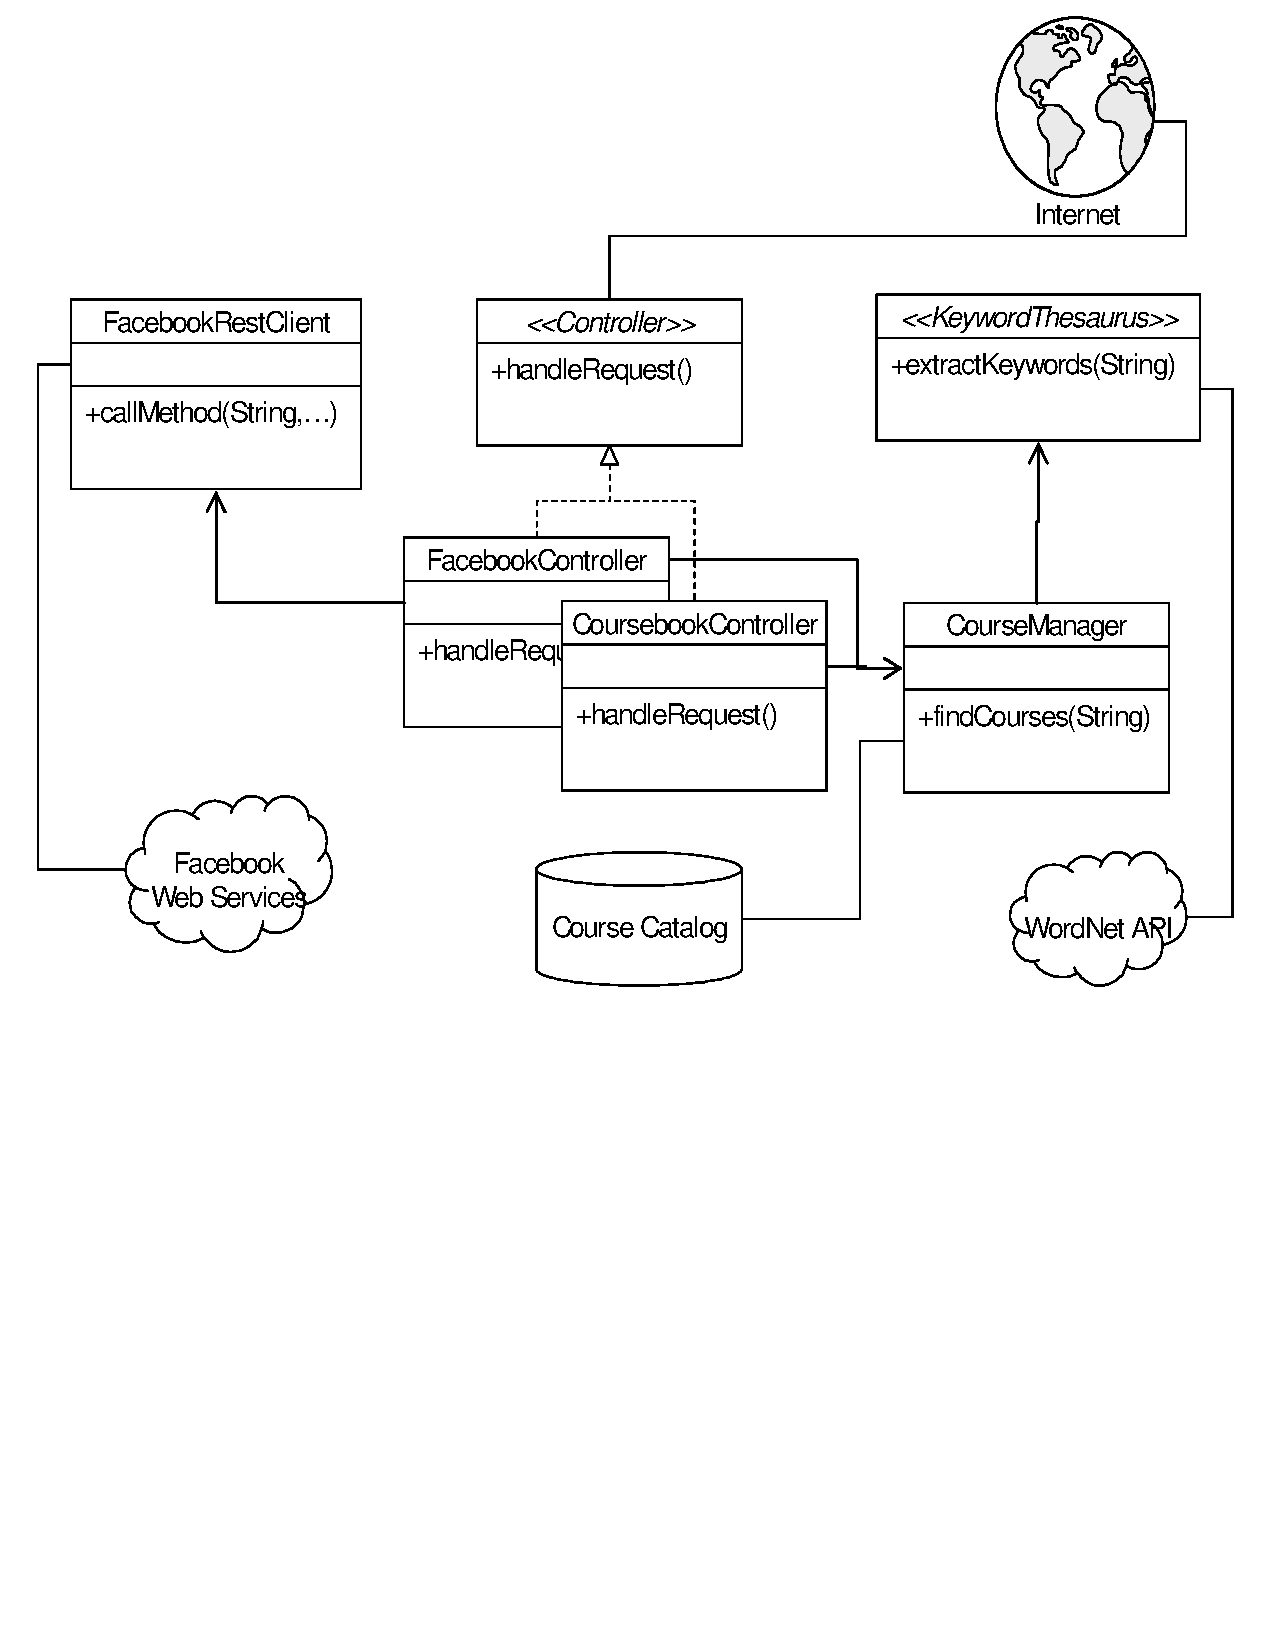
\includegraphics[width=\textwidth]{images/classes}
  \caption{Coursebook Abridged Class Diagram}
  \label{fig:classes}
  \end{center}
\end{figure}

Coursebook makes extensive use of libraries and APIs in its implementation. By
building on several other systems, Coursebook essentially becomes distributed in
the sense that it relies on disparate data sources. First, there is a separate
machine running a database of courses. We also rely on the Facebook web service.
Finally, we use the WordNet API to extract and generate index terms.

Figure \ref{fig:classes} shows an abridged view of the relevant classes used to
construct Coursebook. Initially, user requests come in from the Internet. All
requests are handled by controllers. Coursebook has two such controllers: the
\verb!FacebookController! and the \verb!CoursebookController!. User requests
that provide input through the HTML form come in through the
\verb!CoursebookController!. Users that enter through the Facebook redirection
service (e.g. if they have logged in through Facebook) come in through the
\verb!FacebookController!. This controller uses the Facebook Web Service API to
retrieve profile information from the user's account. Both of these controllers
have a reference to the \verb!CourseManager!. The \verb!CourseManager! is
responsible for querying for relevant courses and their descriptions based on
the user's input. First, the \verb!CourseManager! has access to the course
catalog database. This MySQL database lies on a separate machines and stores all
the information about courses and a index into the courses based on a set of
keywords extracted from their descriptions. Second, the \verb!CourseManager! has
a reference to a \verb!KeywordThesaurus!. This object can extract pertinent  
keywords and find related words based on the pertinent content. This utility is
used to match the user's input with the course database.

These components make up the core distributed functionality of Coursebook. In
later sections, we will describe how we use design patterns within these
components to achieve and improve several quality attributes inside our system. 
